% !TEX program = xelatex
% Draft for author review. Do not submit without attribution and scientific review.
\documentclass{misisarticle}
\grnti{}
\asjc{}
\oecd{}
\title{Восстановление сигнала акселерометра при замирании датчика: ошибка значений и ошибка приращений}
\misisauthor{Кристина Прозорова}{НИТУ МИСИС}{Москва, Россия}{}
\setabstract{На одной реальной записи акселерометра WISDM исследовано восстановление временного ряда после контролируемого замирания измерений. Рассмотрены 32 искусственных повреждения на оси X и три базовых способа заполнения: удержание последнего значения, линейная интерполяция и авторегрессия AR(10). Применены две метрики: RMSE значений и нормированная ошибка первых разностей. Для заранее зафиксированной пары AR(10) и Linear при длине повреждения 200 отсчётов получены средние парные разности $-0{,}840274$~м/с$^2$ и $+0{,}004999$ соответственно. В четырёх из восьми зависимых окон меньшая поточечная ошибка сопровождалась большей разностной ошибкой. Эти оценки характеризуют восемь интервалов одной записи ходьбы.}
\setkeywords{временные ряды, восстановление, измерительные сигналы, акселерометр, авторегрессия, RMSE, первые разности}
\begin{document}
\maketitle

\section{Введение}
Повреждения временных рядов могут приводить к потере отдельных измерений или целых интервалов. Выбор способа восстановления зависит от механизма повреждения, доступной информации и критерия качества. Предыдущие сравнения показывают зависимость результатов от свойств ряда и сценария пропусков~\cite{khayati2020,toye2025}. При этом минимизация ошибки восстановленных \emph{значений} не тождественна минимизации ошибки их \emph{изменений} между соседними отсчётами.

Цель работы --- проверить на одном контролируемом примере акселерометрических измерений, может ли меньший RMSE метода сопровождаться большей ошибкой первых разностей. Единица сравнения --- один и тот же повреждённый интервал, восстановленный двумя способами.

\section{Данные и экспериментальный протокол}
Использована запись телефонного акселерометра из WISDM Smartphone and Smartwatch Activity and Biometrics Dataset~\cite{wisdm2019}. Субъект 1601, активность Walking/A, ось X; строки 1--4512 образуют непрерывный фрагмент из $N=4512$ отсчётов. Изначально наблюдавшийся сигнал $x_i$ служит эталоном \emph{для контролируемого вмешательства}, но не считается доказанно безошибочным физическим измерением.

Для полуоткрытого интервала $I=[s,s+L)$ имитируется замирание оси X:
\begin{equation}
\widetilde x_i=
\begin{cases}
x_{s-1},&s\le i<s+L,\\
x_i,&\text{иначе}.
\end{cases}
\label{eq:freeze}
\end{equation}
Назначенная маска повреждения известна (oracle). Индексы отсчитываются от нуля. Начала интервалов заданы множеством $\{400,800,1200,1600,2000,2400,2800,3200\}$, длины --- множеством $\{5,20,80,200\}$. Всего 32 сценария; вне маски сохранены все исходные значения, включая оси Y и Z. Метки времени не переводились в секунды, так как физическая единица исходного целочисленного поля времени для данной записи не подтверждена.

\section{Базовые методы}
Использованы три неизменяемых после утверждения протокола алгоритма:
\begin{itemize}
\item Hold --- повторение $x_{s-1}$ внутри маски. В этом сценарии результат совпадает с повреждённым сигналом;
\item Linear --- интерполяция между $a=x_{s-1}$ и $b=x_{s+L}$ при $0\le j<L$: $y_{s+j}=a+(j+1)(b-a)/(L+1)$;
\item AR(10) --- модель с десятью лагами и свободным членом, обученная методом наименьших квадратов на 256 предшествующих отсчётах (246 уравнений); прогноз строится рекурсивно с использованием уже вычисленных значений.
\end{itemize}
Linear использует правую границу после повреждения и не сопоставим с Hold и AR(10) по причинному информационному режиму. В каждом сценарии сначала фиксировались предсказания, после чего вычислялись ошибки относительно скрытого эталона. Параметры по исходам данной записи не подбирались.

\section{Метрики и критерий сравнения}
Точность значений на маске определяется RMSE:
\begin{equation}
E=\sqrt{\frac1L\sum_{i=s}^{s+L-1}(y_i-x_i)^2}.
\label{eq:e}
\end{equation}
Для $L\ge2$ обозначим $\Delta x_i=x_{i+1}-x_i$ и $\Delta y_i=y_{i+1}-y_i$. Учитываются только $L-1$ пар внутри маски. Переходы через её границы исключены. Нормированная ошибка приращений равна
\begin{equation}
D=\sqrt{\frac{\sum_{i=s}^{s+L-2}(\Delta y_i-\Delta x_i)^2}
{\sum_{i=s}^{s+L-2}(\Delta x_i)^2}}.
\label{eq:d}
\end{equation}
При нулевом знаменателе $D$ не определена. Для постоянной реконструкции при ненулевых приращениях эталона $D=1$. Это безразмерный индексный показатель, не физическая производная по времени. Дополнительно описано $V=\operatorname{Var}_I(y)/\operatorname{Var}_I(x)$ при ненулевом знаменателе; он не определяет совпадение фазы или формы.

Заранее установленная основная пара --- AR(10) минус Linear при $L=200$. Для каждого из восьми стартов вычислены $\Delta E=E_{\mathrm{AR}}-E_{\mathrm{Linear}}$ и $\Delta D=D_{\mathrm{AR}}-D_{\mathrm{Linear}}$. Совместное разнонаправленное изменение означает $\Delta E<-10^{-10}$ и $\Delta D>10^{-10}$ на одном интервале. Средние вычислены с равным весом восьми стартов. При фиксированной длине интервалы разнесены по одной записи. При одинаковом старте интервалы разных длин вложены друг в друга.

\section{Результаты}
Для всех 32 сценариев получены 96 реконструкций, с точным сохранением значений вне маски. На рис.~\ref{fig:short} и~\ref{fig:long} приведены два заранее фиксированных окна с $s=1200$.

\begin{figure}[htbp]
\centering
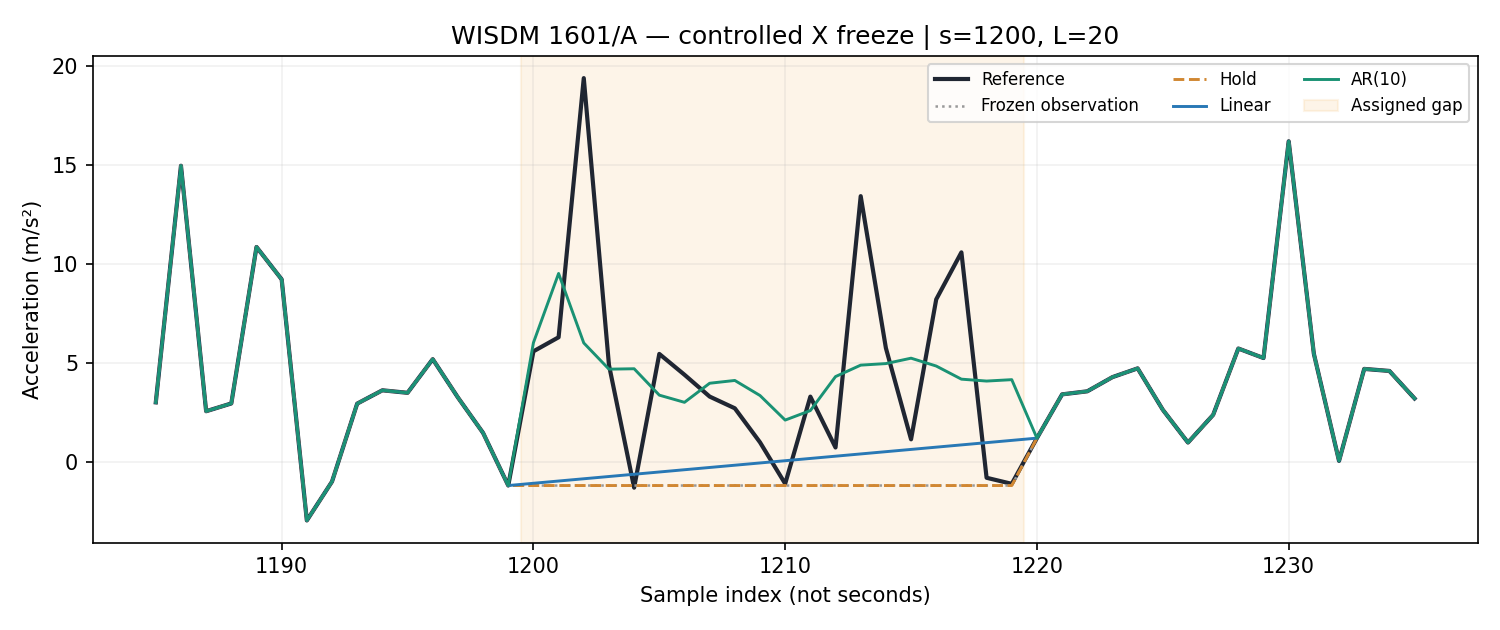
\includegraphics[width=\columnwidth]{figures/repair_s1200_L20.png}
\caption{Один старт, $s=1200$: исходная ось X и три реконструкции короткого интервала ($L=20$).}
\label{fig:short}
\end{figure}

\begin{figure}[htbp]
\centering
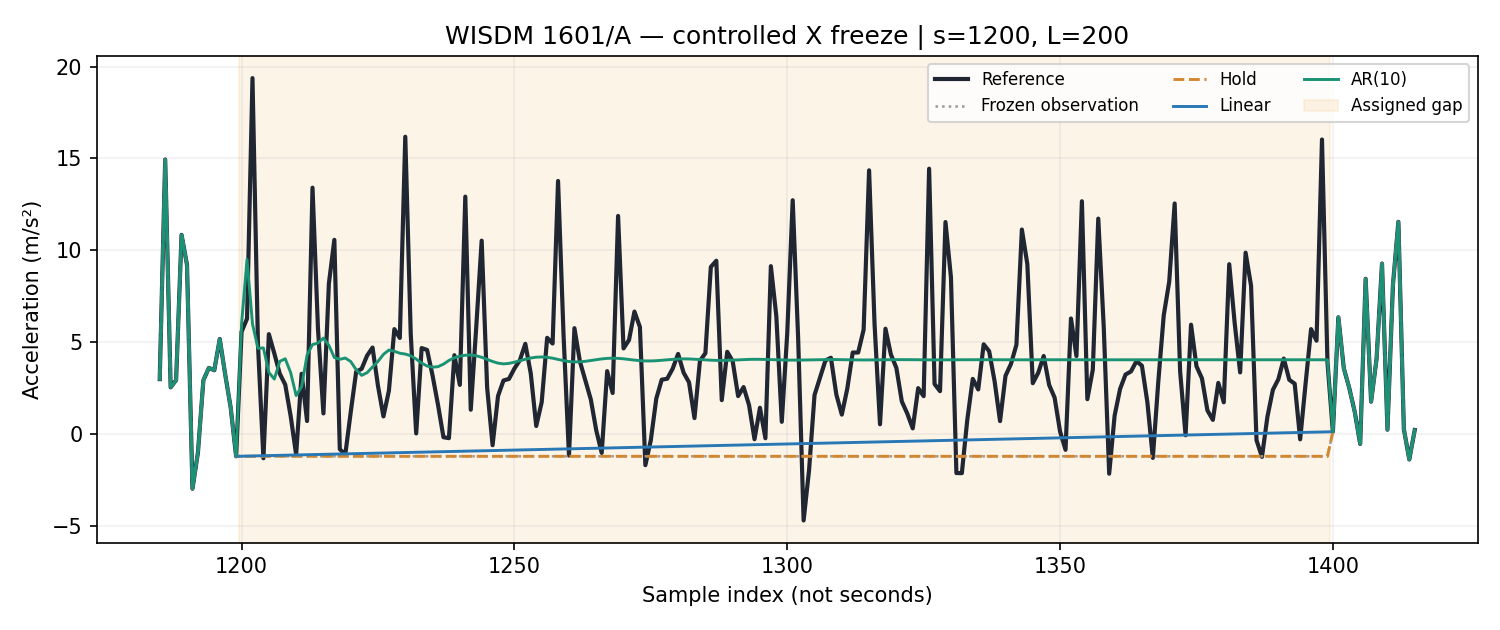
\includegraphics[width=\columnwidth]{figures/repair_s1200_L200.png}
\caption{Восстановление участка длиной 200 отсчётов: затухание прогнозируемых колебаний AR(10).}
\label{fig:long}
\end{figure}

При $s=1200,L=200$ RMSE у AR(10) равен $3{,}756616$~м/с$^2$, у Linear --- $5{,}877733$~м/с$^2$; показатель $D$ составляет $1{,}010637$ против $1{,}000003$. Отношение дисперсий AR(10) равно $V=0{,}01826$, то есть приблизительно $1{,}83\%$ дисперсии исходного фрагмента. Это свойство лишь данного примера.

\begin{table}[htbp]
\caption{Средний RMSE $E$, м/с$^2$}
\label{tab:e}
\centering
\begin{tabular}{rccc}
\toprule
$L$ & Hold & Linear & AR(10)\\
\midrule
5 & 4,9146 & 5,0049 & 3,8134\\
20 & 4,1070 & 4,3427 & 3,3631\\
80 & 3,7615 & 3,6062 & 3,0862\\
200 & 3,6977 & 3,9278 & 3,0876\\
\bottomrule
\end{tabular}
\end{table}

\begin{table}[htbp]
\caption{Средний показатель $D$}
\label{tab:d}
\centering
\begin{tabular}{rccc}
\toprule
$L$ & Hold & Linear & AR(10)\\
\midrule
5 & 1,0000 & 0,9978 & 1,2266\\
20 & 1,0000 & 1,0010 & 1,0224\\
80 & 1,0000 & 1,0000 & 1,0116\\
200 & 1,0000 & 1,0000 & 1,0050\\
\bottomrule
\end{tabular}
\end{table}

Результаты по длинам представлены в таблицах~\ref{tab:e}--\ref{tab:d} и на рис.~\ref{fig:comparison}. При $L=200$ средняя парная разность $E$ для AR(10) и Linear составляет $-0{,}8402744314$~м/с$^2$, или примерно $21{,}4\%$ среднего RMSE Linear. Средняя $\Delta D=+0{,}0049994291$. Все восемь пар имеют отрицательную $\Delta E$; у четырёх положительна $\Delta D$, у остальных четырёх --- отрицательна. На рис.~\ref{fig:paired} показаны эти восемь пар. Среднее изменение $D$ невелико, его статистическая или прикладная значимость не оценивалась.

\begin{figure}[htbp]
\centering
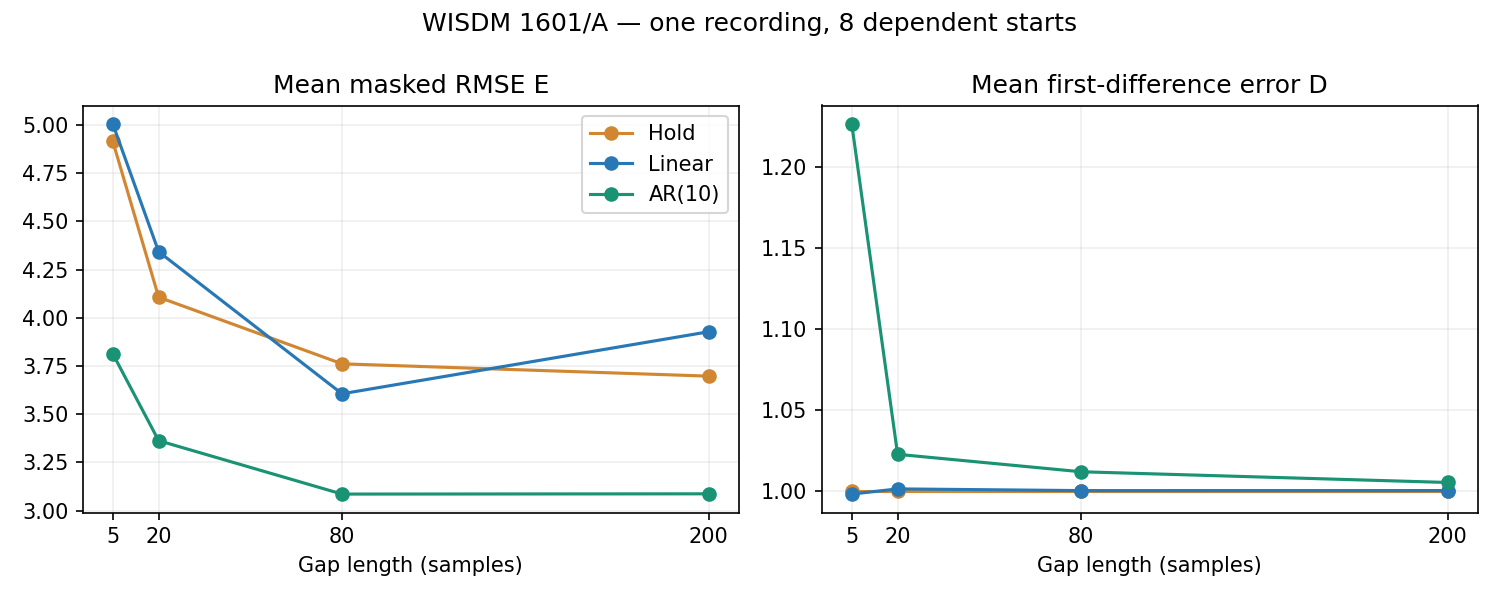
\includegraphics[width=\columnwidth]{figures/comparison.png}
\caption{Оконные средние ошибок по четырём длинам повреждения.}
\label{fig:comparison}
\end{figure}

\begin{figure}[htbp]
\centering
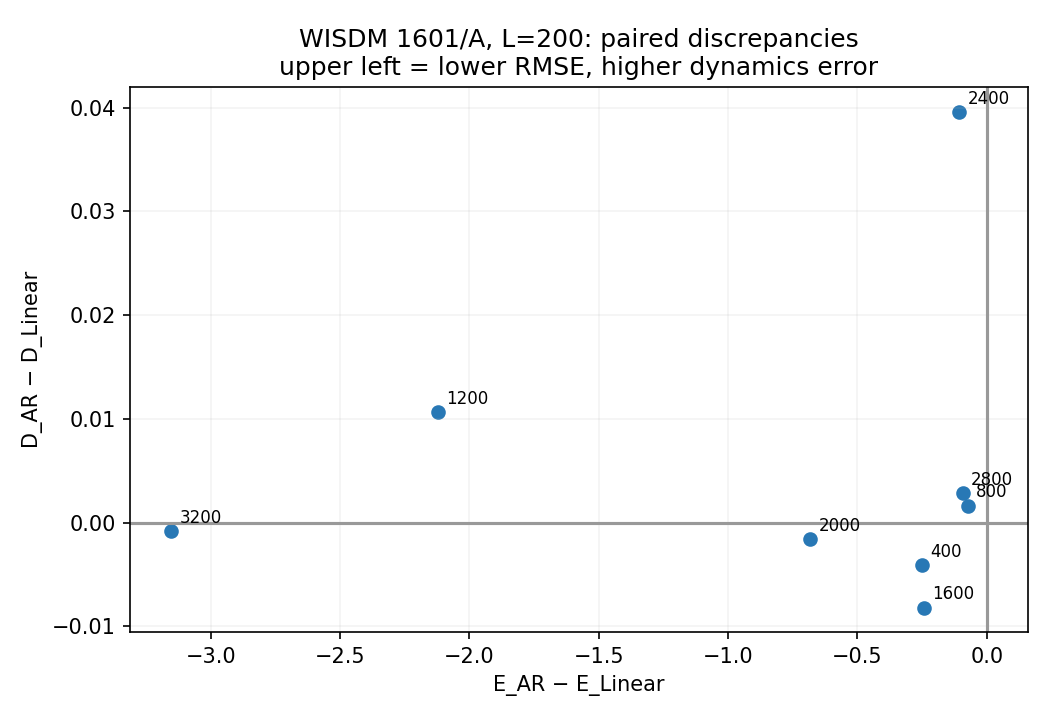
\includegraphics[width=\columnwidth]{figures/paired_L200.png}
\caption{AR(10) минус Linear при $L=200$. Каждая точка соответствует одному старту. Слева от нуля AR(10) точнее по значениям, выше нуля --- менее точен по приращениям.}
\label{fig:paired}
\end{figure}

\section{Обсуждение и ограничения}
На одном наблюдённом ряду продемонстрировано несовпадение двух критериев восстановления: уменьшение ошибок значений может сосуществовать с ухудшением точности приращений. Этот частный результат не устанавливает общую закономерность для других сигналов. Использован один субъект, окна зависимы, ранее проведённые методические обсуждения не гарантируют полностью нетронутого теста: история частного доступа к записи неизвестна. Отказ датчика искусственный, маска известна, а влияние на распознавание активности и спектральную структуру не изучалось.

Различие критериев видно из формул. При ошибке $e_i=y_i-x_i$ числитель под корнем в~(\ref{eq:d}) равен $\sum_{i=s}^{s+L-2}(e_{i+1}-e_i)^2$. Постоянное смещение меняет $E$, но полностью исчезает при взятии разности. Чередование знака ошибки, напротив, увеличивает ошибку приращений даже при небольшой амплитуде.

Khayati и соавт.~\cite{khayati2020} сравнили 12 методов заполнения на десяти наборах рядов. В опытах Toye и соавт.~\cite{toye2025} на рядах глюкозы и пульса линейная интерполяция дала наименьший RMSE при рассмотренных механизмах пропусков. Для актиметрии Weed и соавт.~\cite{weed2022} оценивали сохранение межсуточной стабильности и внутрисуточной вариабельности. В нашем опыте вопрос локален: передаёт ли реконструкция изменение ускорения между соседними отсчётами внутри конкретного интервала?

\section{Заключение}
В фиксированном эксперименте с искусственным замиранием измерений три метода сравнивались по ошибке значений и по нормированной ошибке внутренних приращений. Для одного заранее выбранного сравнения AR(10) уменьшил RMSE относительно интерполяции на всех восьми интервалах длиной 200 отсчётов, но в четырёх из них увеличил разностную ошибку. Это демонстрирует необходимость явно выбирать критерий восстановления по целевой задаче. Расширение вывода на новые субъекты и практические downstream-задачи потребует отдельного протокола.

\begin{thebibliography}{9}
\bibitem{wisdm2019} Weiss G.~M. WISDM Smartphone and Smartwatch Activity and Biometrics Dataset. UCI Machine Learning Repository, 2019. CC BY 4.0. DOI: \url{https://doi.org/10.24432/C5HK59}.
\bibitem{khayati2020} Khayati M., Lerner A., Tymchenko Z., Cudré-Mauroux P. Mind the Gap: An Experimental Evaluation of Imputation of Missing Values Techniques in Time Series. \textit{Proc. VLDB Endow.}, 13(5):768--782, 2020. DOI: \url{https://doi.org/10.14778/3377369.3377383}.
\bibitem{toye2025} Toye A.~A., Celik A., Kleinberg S. Benchmarking Missing Data Imputation Methods for Time Series Using Real-World Test Cases. \textit{Proc. Machine Learning Research}, 287:480--501, 2025. \url{https://proceedings.mlr.press/v287/toye25a.html}.
\bibitem{weed2022} Weed L., Lok R., Chawra D., Zeitzer J. The Impact of Missing Data and Imputation Methods on the Analysis of 24-Hour Activity Patterns. \textit{Clocks \& Sleep}, 4(4):497--507, 2022. DOI: \url{https://doi.org/10.3390/clockssleep4040039}.
\end{thebibliography}
\end{document}
